\documentclass[12pt, a4paper, oneside]{book}
\usepackage{color}
\usepackage{BOONDOX-cal, xeCJK, amsmath, amsthm, amssymb, bm, graphicx, hyperref, mathrsfs, fontspec, subfigure}
\usepackage{pxrubrica}

\graphicspath{{./figures/}}

\title{{\Huge{\textbf{日语学习须知}}}\\——课本上不讲的一些日语小知识}
\author{Alfred}
\date{\today}

\linespread{1.5}
\setCJKmainfont[BoldFont={TH-Hak.TTF}, ItalicFont={TH-Khaai-PP0.TTF}]{TH-Tshyn-P0.TTF}
\setromanfont[Mapping=tex-text]{TH-Times.TTF}
\setsansfont[Mapping=tex-text, Scale=MatchLowercase]{TH-Times.TTF}
\setmonofont[Scale=MatchLowercase]{TH-Times.TTF}
\newtheorem{proposition}{Proposition}[section]
\newtheorem{corollary}{Corollary}[section]
\newtheorem{theorem}{Theorem}[section]
\newtheorem{lemma}{Lemma}[section]
\newtheorem{definition}{Definition}[section]
\newtheorem{example}{Example}[section]
\setCJKfamilyfont{zj}{TH-Ming-P0.TTC}
%\setCJKfamilyfont{hentai}{Zen Kurenaido}
\newcommand{\jp}{\CJKfamily{zj}}
%\newcommand{\hentai}{\CJKfamily{hentai}}
\begin{document}

\maketitle

\pagenumbering{roman}
\setcounter{page}{1}

\begin{center}
    \Huge\textbf{Preface}
\end{center}~\
一门语言的学习涉及多个方面,而教科书上的知识总有未提及的地方,我还是希望能补上这部分的知识。
\\ {\color{red} 注:本书仅对一些内容进行补充,不能单独作为日语学习的教材。}
~\
\begin{flushright}
    \begin{tabular}{c}
        Alfred \
        \today
    \end{tabular}
\end{flushright}

\newpage
\pagenumbering{Roman}
\setcounter{page}{1}
\tableofcontents
\newpage
\setcounter{page}{1}
\pagenumbering{arabic}

\chapter{文字}
日本语使用四种文字:平假名(ひらがな)、片假名(カタカナ)、汉字({\jp \ruby{漢}{かん}\ruby{字}{じ}})和罗马音({\jp ローマ\ruby{字}{じ}})。
\section{书写}
\subsection{平假名}
假名そさきふしりね具有变体写法如下图\ref{tab:dif}。\\
而平假名里面わ行还有两个已经废除的假名ゐ(wi)和ゑ(we),现代日语已经不使用,但是学习古代日语(文语等)还会碰到。在现代日语里ゐ和ゑ一般可以直接认为是い和え。
\begin{figure}[htbp]
\centering
\subfigure[Fuji Mai体]{
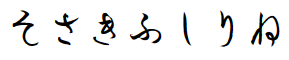
\includegraphics[scale=0.5]{1.png} \label{1}
}
\quad
\subfigure[Zen Kurenaido体]{
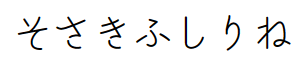
\includegraphics[scale=0.5]{2.png} \label{2} 
}
\quad
\subfigure[Hira Mincho体]{
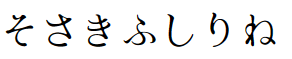
\includegraphics[scale=0.5]{3.png}\label{3}
}
\quad
\subfigure[M Plus 1体]{
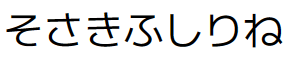
\includegraphics[scale=0.5]{4.png}\label{4}
}
\caption{不同的字体显示的そさきふしりね}
\label{tab:dif}
\end{figure}
\subsection{片假名}
注意ソン以及ツシ两对假名的写法。ソン手写时笔锋朝向不同,ツシ两点相对位置不同,末笔笔锋也不同
\begin{center}
    \textit{\Huge ソンツシ} 
\end{center}
ゐ和ゑ对应的片假名分别是ヰ和ヱ。
\subsection{汉字}
首先声明,日语使用的汉字既不是繁体字也不是简体字,而是日本自己对汉字独立简化后的产物,他们称之为``{\jp \ruby{新字体}{しん|じ|たい}}'',由《{\jp \ruby{当用漢字表}{とう|よう|かん|じ|ひょう}}》规定。而我们所谓繁体字应该被称为``{\jp \ruby{旧字体}{きゅう|じ|たい}}''。\\
而日语的汉字也在一些细节上跟国内不一样。{\jp \color{red}\ruby{結}{むすび}}这个字,就写成{\color{red}\ruby{結}{むすび}}这样也是可以的。但是像{\jp \color{red} \ruby{漢}{かん}}这样的就不能写成汉语{\color{red}漢}这样。这个问题挺复杂的,总之尽量注意一下教材上日语汉字的印刷,有些写法有细微差别。
\subsection{罗马音}
首先也是要强调,罗马音虽然是用拉丁字母(也有人狭隘地称为英语字母或者英文字母)但它纯粹就是一种标记的记号,实际的读音都是有规定的。不能死板地用英语或者汉语(拼音)的读法去套。那么应该怎么读呢?我会在第\ref{chap:prn}章给出一些需要注意的点。但是最好的方法还是去听母语者发音。
\section{一些特殊字符}
\subsection{假名合体字符}
〆乄是しめ合字(前者平假名后者片假);{\jp ゟ}是より合字;ヿ是こと合字;〼是ます合字。
\subsection{重复标记}
々ゝゞヽヾ分别用于汉字、平假名、平假名浊音、片假名、片假名浊音的重复标记。例:{\jp \ruby{時々}{とき|どき}、\ruby{あゝ}{あ|あ}、\ruby{つゞ}{つ|づ}、\ruby{アヽ}{ア|ア}、\ruby{ツヾ}{ツ|ヅ}}。
\subsection{箇}
ヵヶ
\subsection{其他特殊字符}
ヴ行(ヴァ、ヴィ、ヴ、ヴェ、ヴォ)曾经用于直接转写外来语的v发音,现代几乎不使用这种拼写,转用ば行表示,如Videoビデオ。也有使用ウ行转写的Virusウイルス(疫情期间使用量暴增,新冠病毒早期名称就是Novel Corona Virus{\jp \ruby{新型}{しん|がた}コロナウイルス}.
\section{正字法}
虽然日本的新正字法让现代日语读写一致,但是还是保留了一些{\jp \ruby{歴史的}{れき|し|てき}\ruby[g]{仮名}{かな}\ruby{遣}{づか}い}(历史假名用法),导致下面这些现象的发生。
\subsection{はへを}
日语里はへを三个假名由于在语法上同时又是格助词的原因,发音有一点特殊。は作格助词时读作わ,へ作格助词时读作え,を仅作格助词,始终读作お。例句
{\jp \ruby{私}{わたし}は\ruby[g]{昨日}{きのう}\ruby{学校}{がっ|こう}\ruby{校}{こう}へ\ruby{行}{い}って、\ruby{授業}{じゅ|ぎょう}を\ruby{受}{う}けました。}
应该读作{\jp \ruby{私}{わたし}わ\ruby[g]{昨日}{きのう}\ruby{学}{がっ}\ruby{校}{こう}え\ruby{行}{い}って、\ruby{授業}{じゅ|ぎょう}お\ruby{受}{う}けました。}
\subsection{ずづじぢ}
ずづ和じぢ两组假名,每组两个假名读音相同,在现代日语中几乎只使用前者,后者仅在明显是由つ和ち连浊形成时使用。

\chapter{发音}\label{chap:prn}
\section{元音}
元音需要注意的就是う段假名(即罗马音里含有u)的假名。因为う的发音与汉语“呜”有一定差别,发う音时要双唇平行放松,不要嘟嘴,让舌面高点自然地前移,听起来可能有点像“呜”略微偏向“额”的音。其他う段假名同理。\\
需要特别指出假名ふ辅音的发音与汉语“夫”也有所区别,发音时必须让呼出的气从双唇间通过,让上下嘴唇留有空隙才对。
\section{辅音}
\subsection{清浊送气}
要理解日语的发音,就要理解清浊音的概念。\\首先我们得知道,在汉语普通话中是没有浊音的。也正是因为这样,中国人在学习英语等西方语言和日语时,总会碰到一些发音和听力的问题。汉语普通话是区分送气与否的语言,汉语拼音的t和d的区别在于是否送气,而包括英语在内的诸多西方语言和日语都是区分清浊的语言。下面结合国际音标(IPA)进行详细的解说。
\\通俗来说,国际音标是一套用来标记发音的标准符号。而我们使用的拼音,英语法语等使用的音标,日语使用的罗马音等等这些标记发音的方法,都不具有通用性,都是跟其本语言的规定绑定的。而国际音标是大家公认的一个标准,在多语言语音比较,古汉语语音教学中使用较多而平常的语言学习中鲜有介绍。类比一下,长度“米”是国际单位制规定的长度,1米不管在哪个地方他的标准都是一样的,但是各地可能有不同的其他单位,比如里,1里为500米。国际音标也是如此,[t]的发音是固定的,但是在不同语言,其标记可以不同,比如在汉语拼音中用d表记,但英语法语和日语罗马音用t表记。
那么汉语拼音的t用国际音标怎么写呢?答案是[tʰ],但是因为英日等语言不区分送气与否,所以他们也还是认为这个音是t。而他们认为的d(IPA:[d])在汉语普通话里不存在,一般会被视为拼音d。但是这两个音还是有差别的,发[d]时,声带振动,一般发音较低沉;而发[t]时,声带不振动,发音较高亢尖锐。浊音だ[da]和清音た[t]。这也是很多人听{\jp \ruby{私}{わたし}}有听到瓦他西也有听到瓦搭西的原因。\\
在日语中,浊音使用浊音点({\jp \ruby{濁点}{だく|てん}})゛标记。还有一个半浊音点({\jp \ruby{半濁点}{はん|だく|てん}})゜用于ぱ行。在一些具有特殊需求的情况下,可以给か行假名加上半浊音点变成か゚行,表示第\ref{sct:bdo}节中提到的鼻浊音nga。ら行加上半浊音点变成ら゚行,表示la音
\subsection{鼻浊音}\label{sct:bdo}
鼻浊音是一种比较“老”的发音,是が行假名发音[g]的一种变体[ŋ]。这个发音存在于众多汉语方言发音中,但是普通话没有这个音。在汉语里,一般使用ng(ㄫ)表示这个音,在现代中国年轻人中,也有使用嗯表示带有该声母的发音。但是这个音日本年轻人基本不会使用,仅做了解。
\subsection{促音}
促音っ的发音近似为停顿一拍。当碰到っ时,做出其后一个音的口型,不发出声音,近似停顿一拍。但是当后接さ行音时,会自然出现漏气的情况,实际停顿感不明显。
\chapter{输入法}
当使用罗马音输入法时,一般假名使用罗马音打出;单独的拨音ん用nn打出;促音っ用任意非n的辅音双写打出;一般是双写后接的辅音;如って用tte打出;づぢ分别使用du, di打出;ヴ用vu打出。

\end{document}
